Mobile devices in daily life are equipped with more and more powerful computing and storage abilities, which enables individual devices to accumulate more and more valuable information. It facilitates a lot of rising technologies such as edge computing. Meanwhile, the accumulated data in users' devices can be used to train models for various practical purposes due to the flourishing of machine learning. In traditional machine learning frameworks, data needs to be gathered in a central server in order to execute the learning process. However, most data collected by mobile devices is sensitive. Users usually refuse to send their private data to others, such as a learning center, which impedes the development of distributed learning among common users.

Since the computing ability of mobile devices is powerful enough to run small-scale machine learning tasks, federated learning~\cite{mcmahan2016communicationefficient}, which is a distributed machine learning framework, was proposed to address this problem. Figure~\ref{fed} illustrates the structure of federated learning. In each round of FL, parties receive a global model from the server and train their models based on their own data respectively. Afterwards, the parties send the parameters of their models to the server while the server runs a particular aggregation algorithm to compute the global model based on these parameters. In such frameworks, users don't need to send their data to the learning server, and thus privacies of participants are protected.

However, attackers are able to infer users' data through the leaked information of the model's parameters~\cite{Beyond, Leakage, Nasr19}. In the original federated learning framework, parameters are directly sent to the server, which are easy to be captured by others. Therefore, sending parameters to the server directly faces the threat of inference attacks. This kind of attack is quite severe because it can be established by any malicious or semi-honest participant in the federated learning process. Therefore, how to conduct joint learning without leaking parameters to others comes into focus.

Secure aggregation protocols enable a group of parties who have private information to compute a function of these private without revealing them. Researchers paid their attention to secure aggregation for a better solution~\cite{shi2011privacy,RobustAgg,Bonawitz19,Nike,PrivFL}. E.g., Shi et al.\cite{shi2011privacy} utilized homomorphic encryption (HE) methods to achieve secure addition. With the data encrypted, attackers cannot obtain any useful information from leaked messages. Therefore, secure aggregation is suitable for federated learning, which helps to protect intermediate models' parameters. A trivial solution is to employ homomorphic encryption to implement secure aggregation, however, HE algorithms suffer from low efficiency which is hardly acceptable in FL~\cite{HESurvey}. Differential Privacy (DP) is another feasible method to implement secure aggregation whereas DP based frameworks add noises to the parameters to deceive the attackers and these noises also have an influence on the learning result and reduce accuracy. Moreover, Blockchain-based methods~\cite{DeepChain,Lu2020,On-Device} are also very promising, and the generally used consensus algorithms in them can be inspiring. Yet blockchain-based methods are still implement-unfriendly. 

\begin{figure}[!ht]
    \centering
    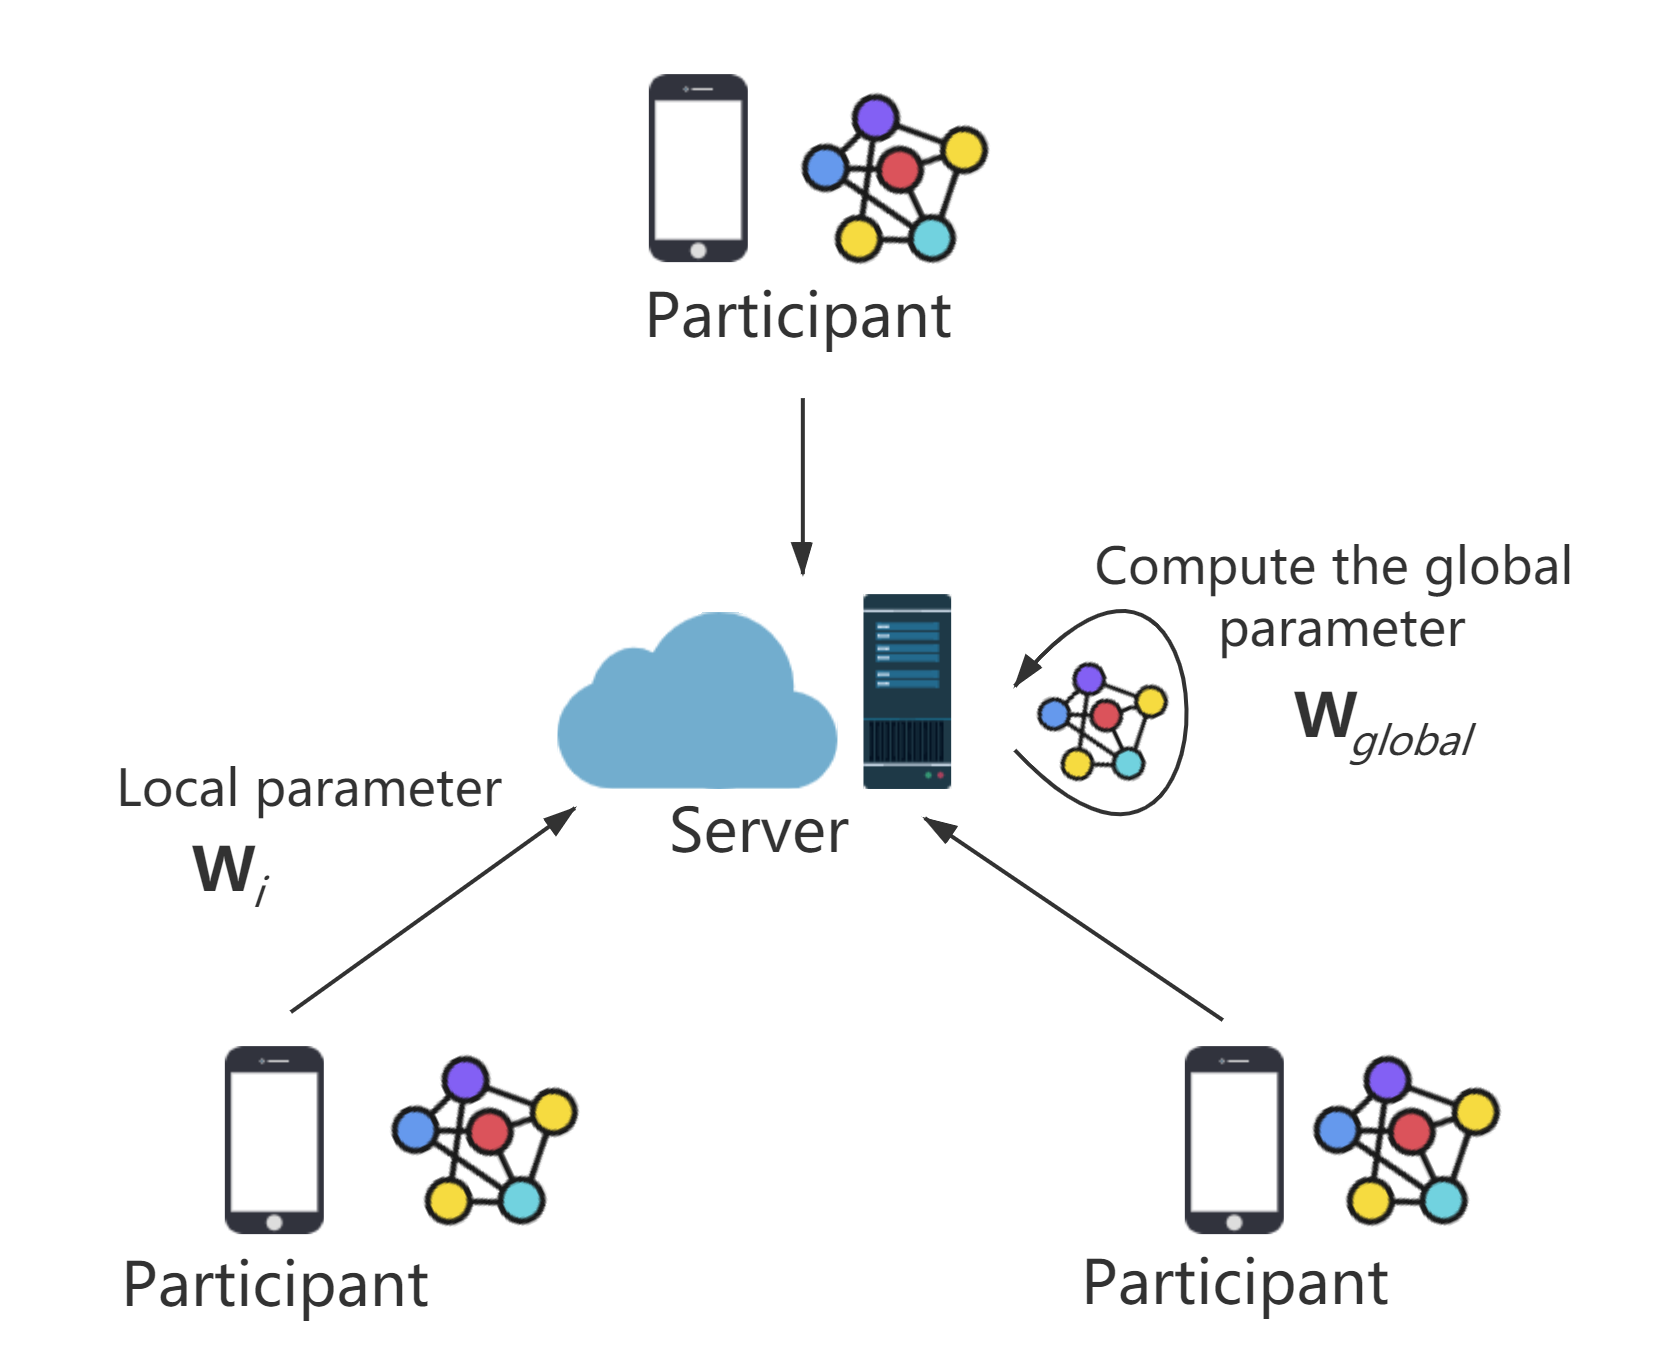
\includegraphics[width=\columnwidth]{img/fed.png}
    \caption{The structure of federated learning. Participants train local models respectively and send their parameters to the server for aggregation.}
    \label{fed}
\end{figure}

One may think MPC is the best method to implement secure aggregation. However, most MPC protocols have a prerequisite: all participants are able to communicate with each other. In practice, common users of a federated learning task are unkown to each other, which means one party cannot communicate with another directly. This is a severe obstacle between MPC and FL. Bonawitz et al.\cite{Practical} utilized Diffie-Hellman key exchange to achieve P2P communication with a dissatisfactory efficiency. As a result, some recent works' attention is on MPC's communication overhead now\cite{Weighted,Two-Phase}. In addition, the robustness of FL frameworks is also significant because it usually costs a lot to recover from situations where several nodes are crashed. And in practice, mobile devices' loss of communication happens frequently, which may cause breakdowns and delays. In summary, employing traditional MPC methods in a system with a large number of users is faced with a problem with efficiency and instability.

% There are 3 primary methods to achieve privacy-preserving in secure aggregation: Differential Privacy (DP), homomorphic encryption, and secure multi-party computation (MPC). DP enabled FL focuses on provides privacy-preserving while keeping the accuracy of the machine learning model. It adds noises to the parameters to deceive the attackers. Whereas, these noises also have an influence on the learning result and reduce accuracy. Since these studies did not conduct experiments with sufficient and complicated machine learning models while some researches have pointed out that DP based FL will impact the accuracy of the learned model~\cite{Two-Phase}, it is still a challenge to employ DP in FL. % HE algorithms are intuitionistic and simple to protect privacy, however, they suffer from low efficiency which is hardly acceptable in FL~\cite{HESurvey}. Even a homomorphic addition will cost too much time thus it cannot reach the requirement of efficiency. Blockchain-based methods~\cite{DeepChain,Lu2020,On-Device} are also very promising, and the generally used consensus algorithms in them can be inspiring. Yet blockchain-based methods are still implement-unfriendly. Therefore, adopting MPC to protect users' privacy is more practical. Many types of research are protecting the parameters based on MPC~\cite{Practical,Two-Phase,Weighted,Hybrid}. 

% Secure multi-party computation can be implemented by garbled circuits or secret sharing methods~\cite{Shamir}. Garbled circuits have many limits and low efficiency. Therefore, we choose to use secret sharing methods. Normally, secret sharing needs parties to exchange information among themselves. However, in federated learning frameworks, the parties are usually strange to each other, which means one party does not have the addresses of others. A party cannot communicate with other parties directly and they can only exchange information securely with the help of the server. In this case, Bonawitz et al.~\cite{Practical} proposed a method about constructing secure channels among FL parties. Constructing secure channels between every pair of parties cost plenty of time, which is a new problem. 

\subsection{Motivation} We aim to design a federated learning framework which has these properties:
\begin{enumerate}
    \item It protects users' privacy by employing MPC, while solving the problem that common users are unknown to each other.

    \item It has low communication overhead, avoiding constructing too many pairwise connections.

    \item It is secure in semi-honest environments, where all users and the server may eavesdrop information.

    \item It is highly robust, which means self-adjusting must be enabled to handle emergencies where several terminals may lose connection.

    \item It does not influence the accuracy of the trained model.
\end{enumerate}

\subsection{Our contribution}
\begin{enumerate}
    \item We propose Self-organizing Federated Learning (SOFL), a novel FL framework that utilizes MPC to protects users' privacy. SOFL employs a simple additive secret sharing protocol to realize MPC, which helps to hide intermediate parameters.

    \item SOFL utilizes hierarchical structure to improve efficiency: our model first elects some leaders, who will construct secure communication with other parties. Afterwards, a party only needs to exchange information with the leaders. The leaders will send the received information to the server, who helps to forward the information to the corresponding destinations. Appointing leaders reduces the need for communications greatly.

    \item We take advantage of consensus algorithm to achieve high robustness. Consensus algorithm helps to handle unexpected situations where a leader node or a common client is crashed. It makes all parties come to an agreement quickly when such situations happen.

    \item We conducted a series of experiments and verified that SOFL has satisfactory efficiency and robustness without reducing accuracy.

\end{enumerate}

\subsection{Roadmap} In Section~\ref{sec:back} we introduce the background of knowledge and some definitions. Next, we introduce related work and some platforms of federated learning in Section~\ref{sec:related}. Section~\ref{sec:sofl} detailedly illustrates our proposed framework while describes the attack model. Evaluations for efficiency and security are stated in Section~\ref{sec:eval}, followed with experiments and results in Section~\ref{sec:exp}. Finally, we give the conclusion and future expectations in Section~\ref{sec:conc}.